\documentclass[aspectratio=169]{beamer}
\usetheme{Madrid}
\usepackage{pifont}  % Подключаем пакет для использования \ding
\usepackage{tikz}
\usetikzlibrary{shapes.geometric, positioning}
\usetikzlibrary{backgrounds}
\usepackage[table]{xcolor}
\usepackage{array}
\usepackage{graphicx}
\raggedbottom

\usepackage[english]{babel}  % Подключение для автоматического переноса слов
\logo{\includegraphics[height=1cm]{logo.png}} % Логотип

\title{JobOsint Bot Presentation}
\author{CEO | Yuriy Galych \newline \texttt{galichy79@gmail.com}}
\date{} % Отключение вывода даты

% Переопределение шаблона footline для удаления email
\setbeamertemplate{footline}
{
  \leavevmode%
  \hbox{%
    \begin{beamercolorbox}[wd=.5\paperwidth,ht=2.25ex,dp=1ex,left]{author in head/foot}%
      \usebeamerfont{author in head/foot} CEO | Yuriy Galych  % Явно указываем имя автора, вместо команды вставки
    \end{beamercolorbox}%
    \begin{beamercolorbox}[wd=.5\paperwidth,ht=2.25ex,dp=1ex,right]{date in head/foot}%
      \usebeamerfont{date in head/foot}\insertframenumber{} / \inserttotalframenumber{}  % Отображение номера слайда
    \end{beamercolorbox}}%
  \vskip0pt%
}
\begin{document}
% Титульный слайд
\begin{frame}
    \centering
    \includegraphics[height=1.5cm]{logo.png} % Логотип центрирован
    \vspace{1cm}
    \titlepage
\end{frame}

\section{Our people may be working for the enemy without even realizing it}

\begin{frame}
    \frametitle{Our people may be working for the enemy without even realizing it}
    
    \begin{block}{Questions that arise when applying for a job}
        \begin{itemize}
            \item Is the company I am going to work for connected to the aggressor country?
            \item Is it a reliable company?
            \item Is it worth getting involved?
            \item Will I have problems because I work or worked for this company?
            \item Etc.
            \item How can I quickly check an employer?
        \end{itemize}
    \end{block}
    
\end{frame}

\section{Our answer is JobOsint Bot}

\begin{frame}
    \frametitle{Our answer is JobOsint Bot}
    
    \begin{block}{AI-based Telegram bot that checks employers using OSINT methods}
        \begin{itemize}
            \item Find job postings of your employer on .ru and .by websites
            \item Analyze employer connections with the aggressor country using OSINT methods
        \end{itemize}
    \end{block}
    
\end{frame}

\section{It takes just 3 simple steps to get started:}

\begin{frame}
    \frametitle{It takes just 3 simple steps to get started:}
    
    \begin{block}{Enter company, enter job title. Get results.}
        \begin{itemize}
            \item Enter company name
            \item Enter job title
            \item Get results
        \end{itemize}
    \end{block}
    
\end{frame}

\section{Market size: Ukrainian and Friends of Ukraine}

\begin{frame}
    \frametitle{Market size: Ukrainian and Friends of Ukraine}

    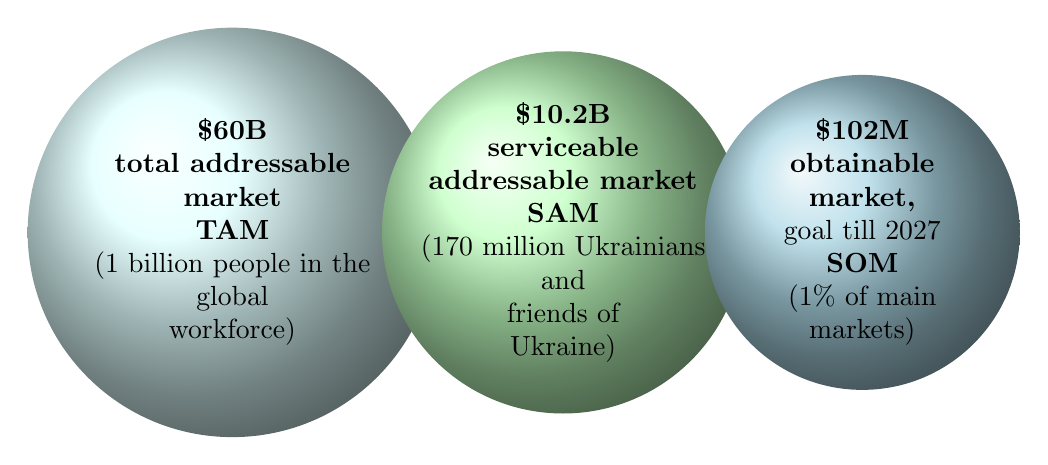
\begin{tikzpicture}

    % Colors for the circles
    \definecolor{lightblue}{RGB}{173,216,230}
    \definecolor{lightgreen}{RGB}{192,255,192}
    \definecolor{lightcyan}{RGB}{224,255,255}
    
    % TAM Circle
    \shade[ball color=lightcyan] (-11.7,0) circle (2.6cm);
    \node at (-11.7,0) {\parbox{4cm}{
        \centering
        \textbf{\$60B}\\
        \textbf{total addressable market}\\
        \textbf{TAM}\\
        (1 billion people in the global\\
        workforce)
    }};

    % SAM Circle
    \shade[ball color=lightgreen] (-7.5,0) circle (2.3cm);
    \node at (-7.5,0) {\parbox{4cm}{
        \centering
        \textbf{\$10.2B}\\
        \textbf{serviceable addressable market}\\
        \textbf{SAM}\\
        (170 million Ukrainians\\
        and\\
        friends of\\
        Ukraine)
    }};

    % SOM Circle
    \shade[ball color=lightblue] (-3.7,0) circle (2cm);
    \node at (-3.7,0) {\parbox{3cm}{
        \centering
        \textbf{\$102M}\\
        \textbf{obtainable market,}\\
        goal till 2027\\
        \textbf{SOM}\\
        (1\% of main markets)
    }};
    
    \end{tikzpicture}

\end{frame}

\section{How do we make money}

\begin{frame}
    \frametitle{How do we make money}
    
    \begin{tikzpicture}
        \node at (0,0) { % Центрируем по координатам (0,0)
            \begin{tikzpicture}
                % Первая карточка
                \shade[left color=green!30, right color=blue!30, rounded corners] (-5,0) rectangle (-0.5,7); % Карточка слева
                \draw[rounded corners, line width=1pt] (-5,0) rectangle (-0.5,7); % Рамка
                \node[align=center, text width=4cm, font=\bfseries, anchor=north] at (-2.75,6.5) {For free};
                \node[align=center, text width=4cm, font=\Large, anchor=north] at (-2.75,5.5) {\$0/mo};
                \node[align=center, text width=4cm, font=\small] at (-2.75,4) {The bot \\ displays ads};
    
                % Вторая карточка
                \shade[left color=green!30, right color=blue!30, rounded corners] (0.5,0) rectangle (5,7); % Карточка справа
                \draw[rounded corners, line width=1pt] (0.5,0) rectangle (5,7); % Рамка
                \node[align=center, text width=4cm, font=\bfseries, anchor=north] at (2.75,6.5) {Premium};
                \node[align=center, text width=4cm, font=\Large, anchor=north] at (2.75,5.5) {\$5/mo};
                \node[align=center, text width=4cm, font=\small] at (2.75,4) {Advanced features \\ available};
            \end{tikzpicture}
        };
    \end{tikzpicture}
    
\end{frame}

\section{Competition}

\begin{frame}
    \frametitle{Competition}
    
    \begin{table}[ht]
        \centering
        \begin{tabular}{|>{\raggedright\arraybackslash}m{2cm}|>{\centering\arraybackslash}m{2.5cm}|>{\centering\arraybackslash}m{2.5cm}|>{\centering\arraybackslash}m{2.5cm}|}
        \hline
        \rowcolor{white} \textbf{Feature} & \textbf{\textcolor{orange}{Osint Bot}} & \textbf{Google} & \textbf{Chat GPT} \\
        \hline
        Available for telegram users & \cellcolor{green!10} Yes & \cellcolor{red!10} Additional registration required & \cellcolor{red!10} Additional registration required \\
        \hline
        No additional registration required & \cellcolor{green!10} Yes & \cellcolor{red!10} No & \cellcolor{red!10} No \\
        \hline
        Integrated with telegram & \cellcolor{green!10} Yes & \cellcolor{red!10} No & \cellcolor{red!10} No \\
        \hline
        Always at hand & \cellcolor{green!10} Yes & \cellcolor{red!10} No & \cellcolor{red!10} No \\
        \hline
        \end{tabular}
    \end{table}
    
\end{frame}

\section{Go to market strategy}

\begin{frame}
    \frametitle{Go to market strategy}

    \begin{tikzpicture}
         
    % Первая карточка
    \draw[rounded corners, thick] (0, 0) rectangle (3, -6);
    
    % Вставляем изображение с сдвигом на 1 см вверх
    \node[align=center] at (1.5, -1) {\includegraphics[width=2cm]{1.png}};  % Сдвиг изображения

    % Текстовые элементы
    \node[align=center] at (1.5, -3) {\textbf{Initial User}\\\textbf{Acquisition}};
    \node[align=center] at (1.5, -5) {Attract our first \\ adoptive users via \\ LinkedIn \\
    Freelancer.com};

    % Вторая карточка
    \draw[rounded corners, thick] (4, 0) rectangle (7, -6);  % Сдвигаем карточку вправо
  
    % Вставляем изображение с сдвигом на 1 см вверх
    \node[align=center] at (5.5, -1) {\includegraphics[width=2cm]{gads.png}};  % Сдвиг изображения

    % Текстовые элементы
    \node[align=center] at (5.5, -3) {\textbf{Google Ads}\\\textbf{Campaigns}};
    \node[align=center] at (5.5, -5) {Target traffic \\ via Google Ads}; 

    % Третья карточка
    \draw[rounded corners, thick] (8, 0) rectangle (11, -6);  % Сдвигаем карточку вправо
  
    % Вставляем изображение с сдвигом на 1 см вверх
    \node[align=center] at (9.5, -1) {\includegraphics[width=2cm]{social.png}};  % Сдвиг изображения

    % Текстовые элементы
    \node[align=center] at (9.5, -3) {\textbf{Social Media}\\\textbf{Advertising}};
    \node[align=center] at (9.5, -5) {Run ads on \\ Facebook \\and Instagram};

    \end{tikzpicture}

\end{frame}

\section{Our team}

\begin{frame}
    \frametitle{Our team}
    
    \begin{columns}
         
        \begin{column}{0.5\textwidth}
            % Рамочка для фотографии
            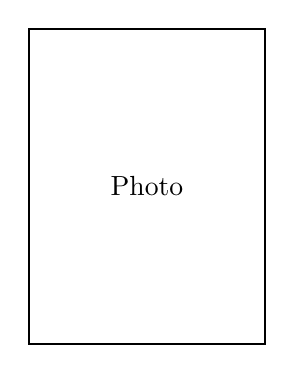
\begin{tikzpicture}
                \draw[thick] (0,0) rectangle (3,4); % Размер рамки (3x4 cm)
                \node at (1.5,2) {Photo}; % Текст внутри рамки
            \end{tikzpicture}
            \vspace{1cm}
            \begin{itemize}
                \item Yuriy Galych - CEO
                \begin{itemize}
                    \item Python developer
                    \item Civil Engineer
                \end{itemize}
            \end{itemize}
        \end{column}
        
        \begin{column}{0.5\textwidth}
            % Рамочка для фотографии
            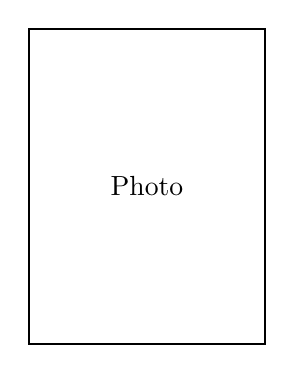
\begin{tikzpicture}
                \draw[thick] (0,0) rectangle (3,4); % Размер рамки (3x4 cm)
                \node at (1.5,2) {Photo}; % Текст внутри рамки
            \end{tikzpicture}
            \vspace{1cm}
            \begin{itemize}
                \item Yana Anisimova - CTO
                \begin{itemize}
                    \item Python developer
                    \item Web Developer with 14+ years of freelancing experience
                \end{itemize}
            \end{itemize}
        \end{column}

    \end{columns}
    
\end{frame}

\section{Money raising}

\begin{frame}
    \frametitle{Money raising}
   
    
    
        
\begin{tikzpicture}
            % Цвета
            \definecolor{orange}{RGB}{255,138,61}
            \definecolor{black}{RGB}{0,0,0}
            
            % Текст
            \node[align=left] at (0,0) {
                \textbf{\textcolor{orange}{\$250K}} \textbf{for the next \textcolor{orange}{18 months} to advance technology and boost}  \textbf{marketing efforts}
            };
            
        \end{tikzpicture}

        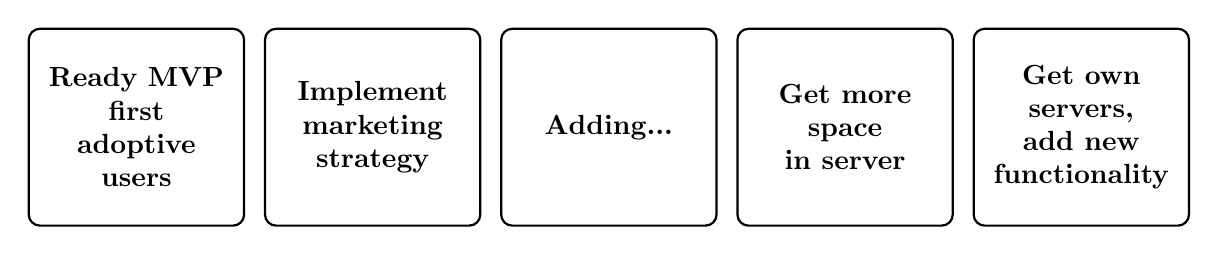
\begin{tikzpicture}
    
            % Определение стиля для карточек с уменьшенными размерами
            \tikzstyle{card} = [rectangle, draw=black, thick, rounded corners, 
                                minimum width=2.5cm, minimum height=2.5cm, 
                                align=center, text width=2.5cm, font=\bfseries]
            
            % Первая карточка
            \node[card] (card1) at (-6,0) {\textbf{Ready MVP} \\ first \\ adoptive \\ users};
            
            % Вторая карточка
            \node[card] (card2) at (-3,0) {Implement \\ marketing \\ strategy};
            
            % Третья карточка
            \node[card] (card3) at (0,0) {Adding...};
            
            % Четвёртая карточка
            \node[card] (card4) at (3,0) {Get more space \\ in server};
            
            % Пятая карточка
            \node[card] (card5) at (6,0) {Get own servers, \\ add new \\ functionality};
        
        \end{tikzpicture}


        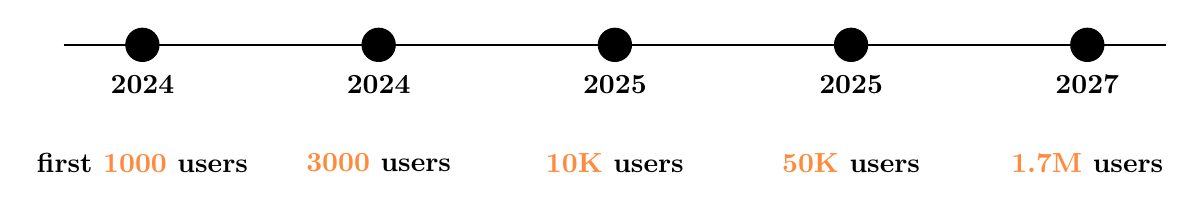
\begin{tikzpicture}
    
            % Цвет
            \definecolor{orange}{RGB}{255,138,61}
            
            % Линия времени
            \draw[thick] (-7,-2) -- (7,-2); % Линия от -7 до 7
            
            % Черные круги на линии времени, выровненные напротив карточек
            \filldraw[black] (-6,-2) circle (6pt); 
            \filldraw[black] (-3,-2) circle (6pt);
            \filldraw[black] (0,-2) circle (6pt);
            \filldraw[black] (3,-2) circle (6pt);
            \filldraw[black] (6,-2) circle (6pt);
            
            % Подписи под кругами
            \node at (-6,-2.5) {\textbf{2024}};
            \node at (-3,-2.5) {\textbf{2024}};
            \node at (0,-2.5) {\textbf{2025}};
            \node at (3,-2.5) {\textbf{2025}};
            \node at (6,-2.5) {\textbf{2027}};
            
            % Текст с чередованием цветов, размещенный ниже
            \node at (-6,-3.5) {\textbf{first \textcolor{orange}{1000} users}};
            \node at (-3,-3.5) {\textbf{\textcolor{orange}{3000} users}};
            \node at (0,-3.5) {\textbf{\textcolor{orange}{10K} users}};
            \node at (3,-3.5) {\textbf{\textcolor{orange}{50K} users}};
            \node at (6,-3.5) {\textbf{\textcolor{orange}{1.7M} users}}; 
        
        \end{tikzpicture}

      
        
   
    
\end{frame}

\section{JobOsint Bot invites investors to join us for peace in Ukraine and Europe}
\begin{frame}

    
\begin{tikzpicture}[remember picture,overlay]
    
        % Background wavy lines (optional decoration)
        \foreach \x in {0,...,15} {
            \draw[opacity=0.2, thin, blue!50] (\x,-0.5) -- (\x-2,9);
        }
    
        % Text block centered on the slide (16:9 aspect ratio)
        % Placing each line of text in its own node for better vertical spacing control
        \node[align=center] at ([yshift=2cm]current page.center) {
            \textbf{\textcolor{orange}{\LARGE JOBOSINT BOT}}
        };
        \node[align=center] at ([yshift=1cm]current page.center) {
            \textbf{\textcolor{gray}{\LARGE INVITES INVESTORS TO JOIN US}}
        };
        \node[align=center] at (current page.center) {
            \textbf{\textcolor{gray}{\LARGE IN INNOVATING THE DIGITAL WORLD}}
        };
    
    \end{tikzpicture}
    
    \end{frame}

\end{document}
